%!Tex Program = xelatex
\documentclass[11pt]{article}
\usepackage{fontspec}
\usepackage{xeCJK}
\usepackage{graphicx}
\setmainfont[Mapping=tex-text,BoldFont=WenQuanYi Zen Hei]{WenQuanYi Zen Hei}
\begin{document}
\section{音频回放基本知识}
\subsection{声音的录制与回放}
    声音的基本处理主要分为两个部分:录制(record)和回放(playback)。

    声音的录制简称为录音,指的是将声音记录在某种介质上。由于声音源于振动,所以介质
只需可以记录振动的幅度即可。录制一段时间的声音,只需要将这一段时间内每个时刻声音的振
幅记录下来。录音时每记录一次振幅称作一次采样,单位时间内采样的次数称作采样频频,简
称采样率。采样率的单位是赫兹(Hz)。

    声音的回放简称为放音,指的是将介质上的声音还原为真实的振动的过程。一段录制好的
声音,按照录音时的采样率,顺序的还原每一个采样,就完成了一段声音的回放。

    声音记录的好坏重点在于振幅记录层级数和采样率的大小。层级数指的是介质可以记录的
最大振幅与最小振幅之间,可以分出多少个层次。可以分的层次越多,可以记录声音越精细,当
层级多于人耳可以分辨的最大值,就是说,人耳无法分辨任意两个层级之间的区别时,声音
对于人耳来讲,就可以完美还原了。人耳的可以分辨的层级数小于65536。声音的频率决定
了声音的粗细,采样率越高,可以记录的声音频率越多。人耳可以分辨的频率是20Hz至
20000Hz之间。所以采样率只需可以记录20000Hz以上的频率即可。工业上一般选择采样率为
44100Hz。

\subsection{声音的数字化}
    在非数字化声音前,声间的振幅与频率整体上由录音设备统一提供,但数字化的声音可
以将两者分开来存放。振幅使用数字记录,频率使用多次采样记录下的数字描绘的波形来记
录。

    一次采样的振幅值可以用一个表示振幅大小的数存储,即为一次采样的数据,录音时,
计算机以确定的采样率记录下一系列数据,即为数字音频。回放时以确定的频率将数据还原
成振幅即可。振幅值用二进制整数保存的音频数据称为PCM格式音频。PCM格式音频有一种存
储其方法是将得到的整数直接按采样的顺序记录下来,不对数据做任何变换,得到的数据可
以看作是振幅值随时间的线性变化,所以也称LPCM。一般常见的PCM格式均是以LPCM方式存
储的。
    
    PCM中,振幅值一般使用8位,13位,14位,16位的有符号或无符号整数存储,采样率一
般没有要求,根据需要录制声音的频段进行选取。

\subsection{音频编码}
    音频编码主要是指音频数据的存储格式,LPCM可以认为是一种最简单的音频的存储格式。
但声音的存储会耗费大量存储空间,所以有必要对数据进行编码(一般伴随着压缩),减少空间需求。

    音频编码有很多种,本节只说明ocarina开发中需要了解的二种编码:a-law,mu-law。

    a-law是一种将原始数据(raw)为13位有符号整数,采样率为8000Hz的LPCM转换为8位整数存储的编码方法。在
计算机内,按G.711的要求,转换方法可以使用以下表格表示:
 
\begin{table}[htbp]
{ \tt
\begin{tabular}{|l|l|}
\hline Linear input code &  Compressed code \\
\hline s0000000wxyza &  s000wxyz  \\ 
\hline s0000001wxyza &  s001wxyz  \\
\hline s000001wxyzab &  s010wxyz  \\
\hline s00001wxyzabc &  s011wxyz  \\
\hline s0001wxyzabcd &  s100wxyz  \\
\hline s001wxyzabcde &  s101wxyz  \\
\hline s01wxyzabcdef &  s110wxyz  \\
\hline s1wxyzabcdefg &  s111wxyz  \\
\hline
\end{tabular}
}
\end{table}


其中s为符号位,其他字母表示普通一位二进制数。

    mu-law的变换方法与a-law整体相同,但其原始数据记录振幅值使用的是14位有符号整数。
转换表如下:

\begin{table}[htbp]
{ \tt
\begin{tabular}{|l|l|}
\hline Linear input code  & Compressed code \\ 
\hline s00000001wxyza & s000wxyz \\
\hline s0000001wxyzab & s001wxyz \\
\hline s000001wxyzabc & s010wxyz \\
\hline s00001wxyzabcd & s011wxyz \\
\hline s0001wxyzabcde & s100wxyz \\
\hline s001wxyzabcdef & s101wxyz \\
\hline s01wxyzabcdefg & s110wxyz \\
\hline s1wxyzabcdefgh & s111wxyz \\
\hline
\end{tabular}

    除去符号位,mu-law可以表示的数值范围是0至8191。为了保证数据有效,原始数
据在做变换之前,需加上33(16进制为0x21,在数据值较小时,形式上用两个“1”将wxyz包
住)。所以实际可用上表转换的数据范围是33至8191。转换完成之后,按规定,为将转换
完成的数据用于存储和传输,需将数据按位取反。
}
\end{table}
    

\subsection{wav容器基本信息}
    音频的编码方式有多种,需要一种方式指明一段数据的编码才有利于音频的存储与交流。
使用数据容器可以很好的达到目的。wav文件就是一种数据容器。
    
    wav文件本身是一个基于RIFF定义的块(chunk)而设计出的一个音频数据容器。RIFF块本身
包含二部分:表征自己意义的头和所要存储的数据。wav文件整体上是一个块,而块的数据部分
又包含了指定音频编码格式的“格式”块和真实音频数据的“数据”块。理解wav文件的基本结构后,
可以轻松的读出其中的音频数据。

    wav文件中所有的数据值均以小尾的方式存储,块结构及数据意义见下图:
\begin{table}[htbp]
    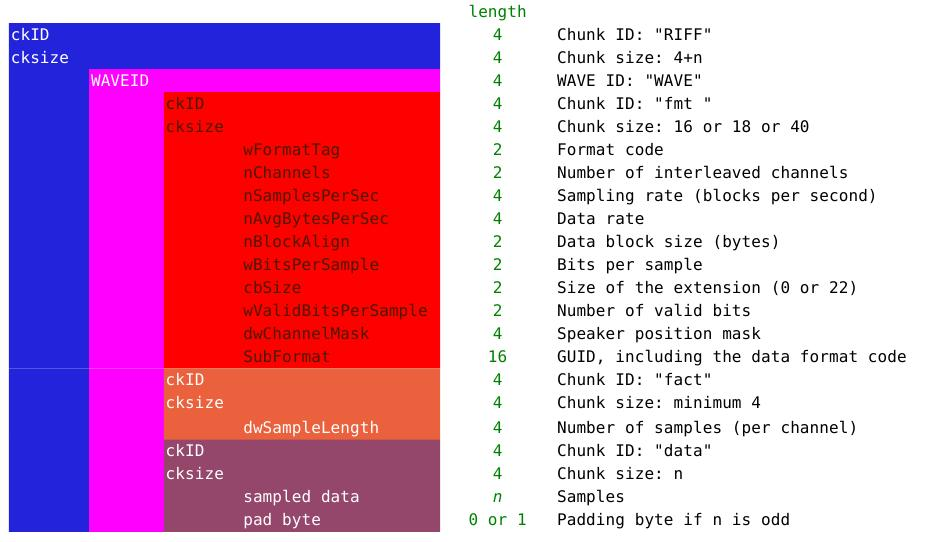
\includegraphics[width = 350pt]{wav_chunk.jpg}
\end{table}



\subsection{RTP的基本信息与承载能力}
    RTP的包头如下表所示:
{  \small
\begin{verbatim}
    0                   1                   2                   3
    0 1 2 3 4 5 6 7 8 9 0 1 2 3 4 5 6 7 8 9 0 1 2 3 4 5 6 7 8 9 0 1
   +-+-+-+-+-+-+-+-+-+-+-+-+-+-+-+-+-+-+-+-+-+-+-+-+-+-+-+-+-+-+-+-+
   |V=2|P|X|  CC   |M|     PT      |       sequence number         |
   +-+-+-+-+-+-+-+-+-+-+-+-+-+-+-+-+-+-+-+-+-+-+-+-+-+-+-+-+-+-+-+-+
   |                           timestamp                           |
   +-+-+-+-+-+-+-+-+-+-+-+-+-+-+-+-+-+-+-+-+-+-+-+-+-+-+-+-+-+-+-+-+
   |           synchronization source (SSRC) identifier            |
   +=+=+=+=+=+=+=+=+=+=+=+=+=+=+=+=+=+=+=+=+=+=+=+=+=+=+=+=+=+=+=+=+
   |            contributing source (CSRC) identifiers             |
   |                             ....                              |
   +-+-+-+-+-+-+-+-+-+-+-+-+-+-+-+-+-+-+-+-+-+-+-+-+-+-+-+-+-+-+-+-+

\end{verbatim}
}

    RTP使用RTP头描述自身信息。因为并不描述包长度,所以适合于UDP传输。RTP头的封装需要
注意几点:
\begin{enumerate}
    \item 所有数值使用网络序
    \item 使用“承载”数据项描述类型
    \item 数据标号用来描述包的顺序,起始值随机,每包增一
    \item 时间戳描述为每个包相对于初始包的采样增量,可以理解为当前包的第一个采
        样在整个音频采样序列中的偏移量。因为RTP可以从任意包开始播放,所以,初始
        包只是一个概念,并不一定真实存在
    \item 时间戳之间的增量,可以在sdp协商中指定。sdp的a属性ptime(packet time),可以指定(按sdp协
        议,此值仅为建议值,板卡可以选择忽略)封包时长,通过封包时长以及承载类型,可以换算
        出每个RTP包可以含的采样数,即为时间戳增量
\end{enumerate}

   RTP详细信息参考RFC3550,不再赘述。

\subsection{整体放音流程}
    处理进程接收指令,将指定铃音文件内所含的音频信息发送至指定端口,自动结束或接收指
令结束放音,是一个完整的放音流程。除去指令处理和系统相关操作,放音流程主要分为三
个部分:从铃音文件中读取音频数据,将数据转化成目标编码,将编码好的数据使用RTP格式
封装,并按RTP定义,每隔指定时间发送至网络。
%\subsection{基本技术点}
%    基本功能需要如下技术点:
%    \begin{enumerate}
%        \item wav中数据的读取
%        \item 编码相关的数据转换
%        \item RTP包头的信息填写
%    \end{enumerate}
%以下给出各技术点的详细信息及建议处理方式。
\subsection{音频数据的读取}
    在了解wav文件格式后,可以从wav文件中将采样率与采样序例读出,即为音频数据。
\subsection{中间格式与转码}
    如果从文件中读出的数据与RTP最终需发送的数据格式不同,则需要经过转码过程。
为增加通用性,转码的方法是将源数据先转换为中间数据格式,再将中间格式转为目标编码。
若目标编解码器未支持但存在开源实现,尽量选用开源的代码。如果开源的代码不能使用,
则需自己开发。编解码所需的内存视编码的方式不同而不同,由于音频数据是线性的,空间
复杂度基本为O(n)。

    建议ocarina选用wav和RTP同时支持的编码,减少中间转码环节,节省开发时间。
基本的wav只支持PCM,a-law,mu-law和实数四种格式。基于RTP的封包要求,建议wav内封装的数据
是8kHz的8bit的mu-law音频。
\subsection{封包时长选取}
   RTP的封包时长可以任意选取。但封包时长越长,丢包时造成的影响越大;封包时长越短,
则数据长度占整个网络数据包长度的比例越小,造成带宽浪费。建议按RFC建议,封包时长选
为20ms。
\subsection{封包时长与数据长度}
   当封包时长选定后,一次数据传送的采样个数就确定了,其值为$$S = F \cdot l/L$$

   其中S是采样的个数,F是采样率,l是封包时长,L采样率基准时间单位,取为1s。

   根据承载类型确定的单个采样的数据长度,即可计算RTP包的数据长度。以mu-law
为例,20ms的采样个数为160,单个采样的数据是1Byte,所以一个封包的数据长度是160Byte。
\subsection{封包过程}
   将需要封包的数据,按照计算得到的采样个数,每次封装所需的采样个数即可。若音
音频结尾,采样数少于所需的采样个数,可以仅封包最后采样。但需循环播放等情况可
能出现时间戳增量不均的情况。建议用静音填充不足的采样。

\subsection{铃音缓存}
    当系统高并发时,有可能出现磁盘响应不足和转码时间超量的性能问题,解决的方法是铃音
缓存。

    铃音缓存指在板卡内部的铃音缓存,与外部缓存无关。板卡内部可以将某些常用的铃音文件
处理后,生成RTP序列,完全缓存在内存中,当有新的请求到来时,可以直接将数据的RTP头修改
为需要的值后直接发送。此方法不会因请求过多而造成内存压力过大,因为所有请求该铃音的进
程可以共享同一副本。现网铃音的数据平均大小为200KB,最长大约为60秒的铃音文件,约480KB,
以平均换算,1GB内存可以存储约5000首铃音。根据现网调研报告,现网运行的采铃系统在缓存
2000至3000首铃音时,命中率即可达到百分之七十至八十,达到二八原则的最优值,同时线网的
服务器可以提供的内存远超1GB,所以缓存策略有效。
\end{document}
